\chapter{Introduction}

\section{Background and Motivation}
Most people who have tried to book an appointment at a local clinic, salon, or therapy center know the routine all too well. A customer calls, often having to try multiple times before getting through, waits on hold while the receptionist checks a physical register, confirms a time, writes it down, and hopes the other side remembers too. Sometimes the appointment goes smoothly, but often it is missed, double-booked, or forgotten because the process depends entirely on manual coordination and human memory. This reliance on outdated methods not only frustrates the customer but also creates unnecessary stress for the business staff, who must constantly juggle ringing phones while trying to serve the clients already present in the establishment.

This problem is extremely common in small and medium-sized service businesses where daily operations are still largely managed through phone calls, paper registers, whiteboards, and informal memory. For example, a salon owner may keep a physical register of appointments, yet still face frequent missed bookings, cancelled slots without prior notice, or confusion over staff availability when multiple employees share the same workspace. Even when digital tools and scheduling software exist in the market, many of them are heavily geared towards large enterprises. They are often too expensive, packed with unnecessary features that make them too complicated to learn, or simply not designed for the specific, agile needs of small local businesses. These local businesses require a straightforward solution that integrates seamlessly into their workflow without requiring extensive technical training.

The motivation for \textbf{Slotify} came directly from observing this significant gap in the market. Small service businesses need a simple, affordable, and reliable online system that helps customers book appointments quickly while letting service providers manage their schedules and resources more efficiently. The core aim of this project is to drastically reduce manual administrative work, completely avoid schedule conflicts like double-bookings, improve transparent communication between the service provider and the client, and provide a significantly smoother, frictionless booking experience for both customers and businesses. By automating the most tedious parts of scheduling, business owners can focus more on delivering high-quality services rather than managing calendars.

\section{Problem Statement}
Manual coordination overhead and appointment attrition are two sides of the same operational issue that continuously plagues service-based industries. When bookings are managed strictly over phone calls, text messages, or handwritten records, every single transaction requires a human in the loop. Someone must explicitly confirm the time, manually record the booking in a ledger, carefully check for potential conflicts across different staff members, and manually follow up with reminders a day before the appointment. This manual approach might work adequately at a very low volume of customers, but it breaks down rapidly and becomes highly error-prone as the business grows and customer demand increases. The sheer volume of communication can overwhelm staff, leading to mistakes that directly impact customer satisfaction.

At the same time, no-shows and empty time slots create direct and irrecoverable revenue loss. Customers frequently forget appointments if they are not reminded, and a last-minute cancellation is almost never re-filled quickly because there is no automated system to notify other waiting customers. Furthermore, the business has no real-time visibility into scheduling gaps or performance metrics. Without automated reminders, waitlists, or digital slot management, small businesses lose valuable time, hard-earned money, and essential customer trust. The unpredictability of daily schedules also makes it difficult to manage staffing levels effectively.

Another major challenge contributing to this problem is that many existing booking systems are architected and priced for large corporate organizations. They simply do not fit the specific, dynamic needs of small businesses such as local salons, dental clinics, wellness centres, and independent tutors. These smaller businesses need flexible calendars that can handle irregular hours, specific staff assignments based on expertise, and a very easy, intuitive process for managing daily appointments without introducing unnecessary technical complexity or requiring dedicated IT support.

\section{Project Objectives}
The main objectives of the project are as follows:

\begin{enumerate}
\item To design and build a highly responsive, customer-facing booking system that allows users to seamlessly search for service providers, view real-time available time slots, and securely book appointments online without any need for manual phone coordination or intervention.
\item To develop a comprehensive and intuitive provider dashboard specifically tailored for business owners and managers. This dashboard must allow them to manage daily schedules, track staff availability, adjust service timings, and monitor overall business operations efficiently from a centralized location.
\item To architect and implement a robust real-time appointment mechanism that strictly prevents double bookings, handles concurrent booking attempts gracefully, and significantly reduces overall schedule conflicts across the platform.
\item To provide a fully automated notification system that instantly sends confirmation emails upon booking and dispatches timely reminder emails prior to the appointment, ensuring that customers do not forget their scheduled times and thereby reducing no-show rates.
\item To create an exceptionally simple, clean, and user-friendly interface for both customers and service providers, minimizing the learning curve and making the platform highly accessible even to users with limited technical proficiency.
\item To support and generate actionable business analytics, providing business owners with clear insights into appointment trends, peak hours, cancellation rates, and workload distribution among staff members, ultimately aiding in better decision-making.
\end{enumerate}

\section{Scope}
The current scope of the project comprehensively covers service-based businesses that operate strictly on a time-slot model. This includes, but is not limited to, medical clinics, beauty salons, tutoring services, repair shops, and physiotherapy centres. The system architecture is designed from the ground up to support a multi-tenant environment, meaning it caters to multiple independent businesses simultaneously, with each business having completely separate data, secure access controls, and customized settings. 

The platform's primary focus in its initial phase is on delivering robust online appointment scheduling, detailed business management features, and automated email notifications. While features such as native mobile applications (for iOS and Android) and integrated in-app payment processing gateways (like Stripe or PayPal) are incredibly valuable, they are intentionally kept outside the scope of the current initial phase to ensure core stability. However, the system is architected with modularity in mind, so these features are actively considered and planned as major future enhancements in subsequent iterations.

\section{System Overview}
\textbf{Slotify} is envisioned as a comprehensive web-based platform that seamlessly connects customers, service providers, and business administrators through a single, unified scheduling system. From the customer's perspective, they can easily browse through various listed services, check the real-time availability of their preferred providers, and securely book appointments after selecting suitable time slots that fit their schedule. On the other side, service providers and business owners can meticulously manage their daily working hours, assign specific staff members to different services, block out holidays, and monitor all incoming bookings from a dedicated, interactive dashboard.

The system is meticulously designed to handle the entire lifecycle of a booking. This begins with service discovery and intelligent slot selection, moves through the secure confirmation process, and concludes with automated reminder notifications sent directly to the user's inbox. Beyond just handling individual appointments, the platform also heavily supports business-level data tracking. By aggregating scheduling data, it makes it significantly easier for business owners to understand their busiest periods, track staff performance, and make informed operational decisions that can drive growth.

The core philosophy and key idea behind the system's architecture is to deeply automate the intricate scheduling process while keeping the user interface as simple, clean, and accessible as possible. This deliberate focus on user experience reduces the administrative effort required by the business to almost zero and creates a highly professional, frictionless, and modern experience for the end customers, elevating the business's overall brand perception.

\begin{figure}[h]
\centering
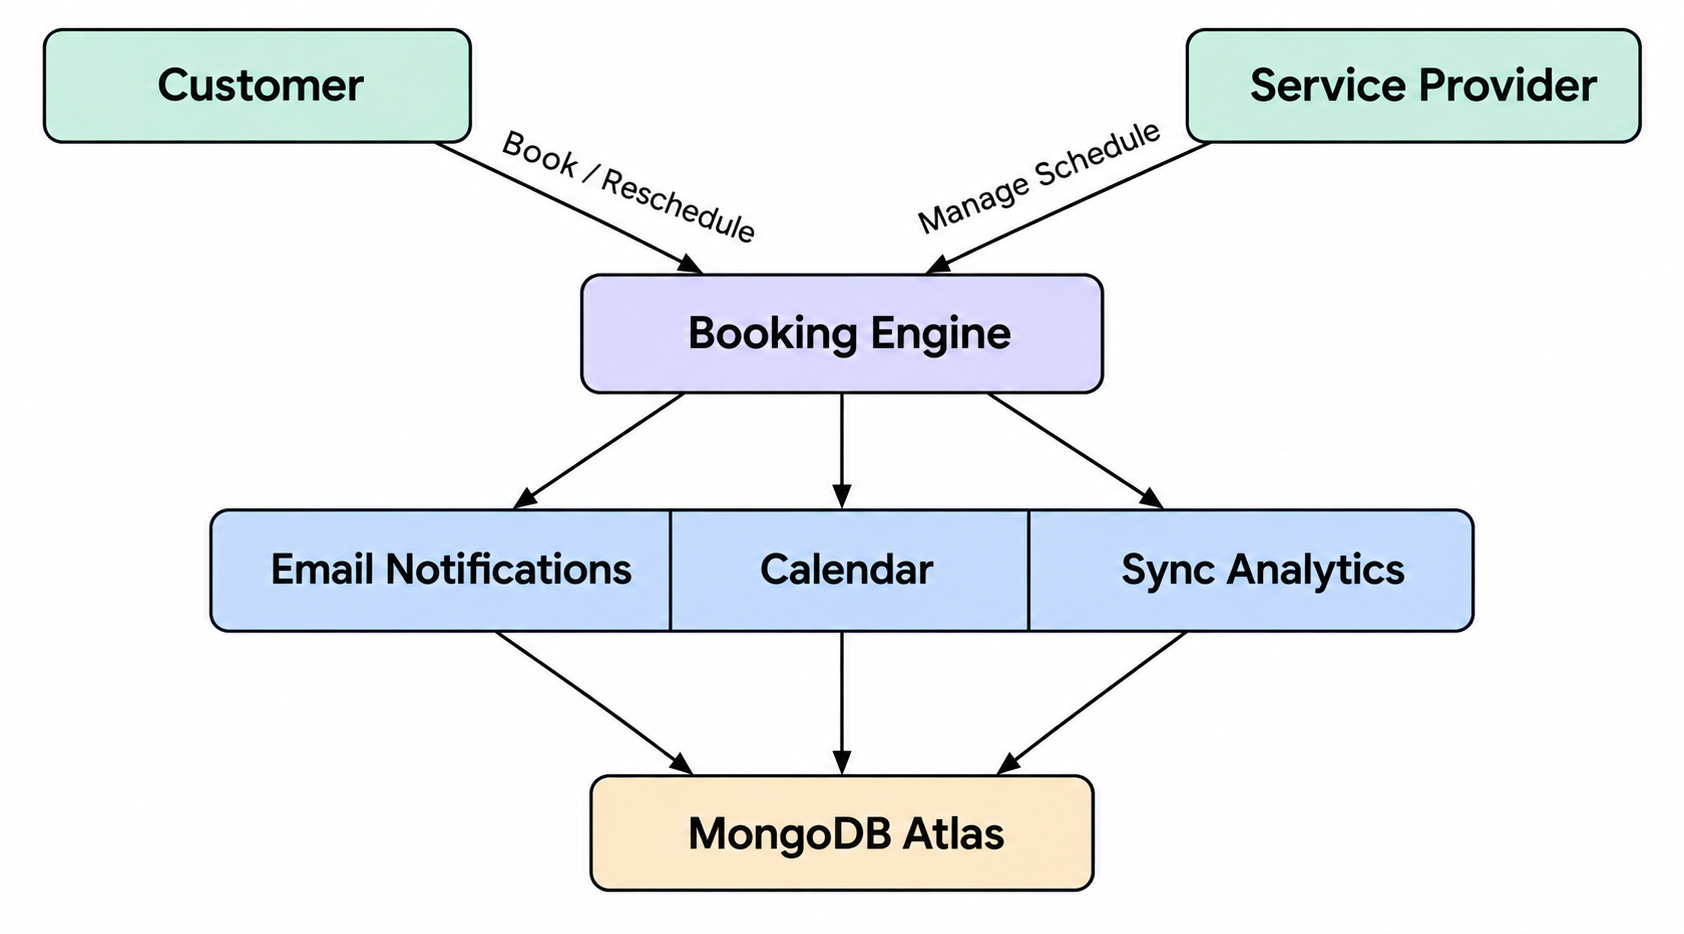
\includegraphics[width=\textwidth]{images/figure 1-1.png}
\caption{System overview of the Slotify appointment workflow}
\end{figure}

\begin{table}[h]
\centering
\caption{Key scheduling challenges and their solutions in Slotify}
\begin{tabular}{|p{5cm}|p{7cm}|}
\hline
\textbf{Problem} & \textbf{How Slotify solves it} \\
\hline
Double booking & Real-time slot checking and conflict prevention during appointment creation \\
\hline
Missed appointments & Confirmation emails and reminder notifications sent to customers \\
\hline
Manual coordination & Digital booking system reduces dependence on phone calls and paper records \\
\hline
Low business visibility & Dashboard tracks bookings, workload, and appointment trends \\
\hline
\end{tabular}
\end{table}

\section{Technology Stack}
The project is developed using the widely adopted MERN stack, which provides a highly flexible, robust, and scalable foundation for building modern web applications. The choice of this stack allows for seamless data flow using JavaScript across both the client and server sides. The stack includes:

\begin{itemize}
\item \textbf{MongoDB}: A powerful, document-oriented NoSQL database used to flexibly store complex hierarchical data such as business details, user profiles, dynamic appointments, customizable services, and historical booking records. Its schema-less nature allows for rapid iteration during development.
\item \textbf{Express.js}: A minimal and flexible Node.js web application backend framework that provides a robust set of features for web and mobile applications. It is used to define clear RESTful APIs, manage complex routing, and handle server-side business logic efficiently.
\item \textbf{React.js}: A declarative, efficient, and flexible frontend JavaScript library used to build the interactive user interface. It enables the creation of reusable UI components, ensuring a highly responsive and dynamic user experience across different devices and screen sizes.
\item \textbf{Node.js}: An asynchronous, event-driven JavaScript runtime environment designed to build scalable network applications. It is used for server-side execution, handling multiple concurrent connections with high throughput and low latency.
\end{itemize}

The application also securely integrates advanced authentication mechanisms such as JWT (JSON Web Tokens) for session management and Google OAuth for streamlined, secure login and user verification, reducing the friction of creating new accounts. Appointment notifications and system alerts are sent using Nodemailer, which enables reliable, real-time email confirmations and automated reminder messages directly from the server. This precise combination of modern web technologies ensures that the system is not only scalable to handle high traffic but also secure against common web vulnerabilities, and easy to maintain and extend in the future.

In summary, \textbf{Slotify} directly addresses the critical, everyday scheduling challenges faced by small and medium-sized service businesses by delivering a fully digital, highly automated, and exceptionally user-friendly appointment booking solution that transforms how they interact with their clientele.
